\documentclass{beamer}
\usepackage[russian]{babel}
\usetheme{metropolis}

\usepackage{amsthm, amssymb}
\setbeamertemplate{theorems}[numbered]

\setbeamercolor{block title}{use=structure,fg=white,bg=gray!75!black}
\setbeamercolor{block body}{use=structure,fg=black,bg=gray!20!white}

\usepackage[T2A]{fontenc}
\usepackage[utf8]{inputenc}

\usepackage{hyphenat}
\usepackage{amsmath}
\usepackage{graphicx}

\AtBeginEnvironment{proof}{\renewcommand{\qedsymbol}{}}{}{}

\title{
Микроэкономика-I
}
\author{
Павел Андреянов, PhD
}

\begin{document}

\maketitle

\section{Программа курса}

\begin{frame}{Программа модуля}
\begin{itemize}
\item Теория Потребителя
\begin{itemize}
\item Модель: товары $x, y$ $\to$ полезность $U(x,y)$
\item Максимизация полезности
\item Предпочтения, спрос, эластичность...
\item CV, EV
\end{itemize}
\item Теория Производителя
\begin{itemize}
\item Модель: ресурсы $x, y$ $\to$ производство $F(x,y)$
\item Максимизация прибыли (минимизация издержек)
\item Технологии, предложение, эластичность...
\end{itemize}
\item Частичное равновесие
\begin{itemize}
\item налоги, потолки, DWL
\end{itemize}
\end{itemize}
\end{frame}

\begin{frame}{Люди и материалы}

Лектор: Павел Андреянов (pandreyanov@gmail.com/hse.ru)

Семинаристы: Даша

Учебники:
\begin{itemize}
\item Вэриан (V) и Ехил Рени (JR), есть русские версии
\item Бусыгин, Желободько, Цыплаков (BZC) том I,II
\item Мас Колел (MC)
\end{itemize}

Задачник -- Левина, Покатович

\end{frame}

\begin{frame}{Люди и материалы}

Прочие ресурсы:
\begin{itemize}
\item телеграм: \url{channel_micro_2023}, \url{forum_micro_2023}
\item офис аурз: TBD
\item консультации и тестовые контрольные
\item \url{pandreyanov.github.io/pashas_micro_one_lectures}
\end{itemize}

\end{frame}

\begin{frame}{Люди и материалы}

\begin{figure}[hbt]
\centering

\includegraphics[width=.6 \textwidth]{qrcode}
\end{figure}

\end{frame}

\section{Предисловие}

\begin{frame}{Предисловие}

Экономика это не физика, и не ветвь прикладной математики, а школа философской мысли, в которой некоторые рассуждения могут делаться при помощи математики. 

Но на сегодняшний день традиция такова, что мы думаем об экономике именно в терминах жестких математических моделей. 

\end{frame}

\begin{frame}{Предисловие}

Модели пишутся на языке мат. анализа, что позволяет этим моделям пересекать временные, языковые и культурные границы. 

Но само по себе использование мат. анализа не делает эти модели <<правильными>>  и, в конечном счете, оценка качества модели субъективна.

В экономике вообще нет <<правильных>> моделей. 

\end{frame}
%
%\begin{frame}{Предисловие}
%
%За последние полвека в экономике было создано большое количество конкурирующих моделей, некоторые из них открыто противоречащих друг другу. Эти модели постоянно обновляются, сменяют друг друга. 
%
%Это не признак незрелости экономической науки а, наоборот, ее достижение. 
%
%\end{frame}
%
%\begin{frame}{Предисловие}
%
%В физике такое случалось всего несколько раз и это чуть не привело к кризису  научной мысли. Например, Эйнштейн отказывался верить в то, что нет   <<правильной>> модели, объясняющей все наблюдаемые квантовые парадоксы. 
%
%Он утверждал, что через какое-то время нужная модель найдется, надо только подождать.
%
%\end{frame}
%
\begin{frame}{Предисловие}

Существует большое количество разнообразных моделей и у каждой есть свои достоинства и ограничения.

В этом курсе мы научим вас быть последовательными в рамках отдельно взятых моделей, а также немного разбираться в их многообразии.

\end{frame}

\section{План}

\begin{frame}{План на первую половину лекции}

\textbf{Модели поведения потребителя.}

Мы поговорим подробно о первых двух моделях (полезность и предпочтения) и, вскользь о третьей модели (выбор). Большой упор будет сделан на понятия непрерывности и выпуклости. (\alert{скорее всего тут время закончится})

Затем, мы попробуем отождествить некоторые из этих моделей между собой. В частности, будет обсуждена относительно простая прямая связь между полезностью и предпочтениями.

Вершиной этого блока будет обратная связь между предпочтениями и полезностью, так называемая, \alert{Теорема Дебре}. После нее надо сделать перерыв.

\end{frame}

\section{Что такое модель?}

\begin{frame}{Что такое модель?}

Модель - это упрощенная версия реальности, из которой специально убраны детали, иногда очень важные, для того чтобы изолировать и анализировать какой то один аспект этой (сложной) реальности. 

Сила модели идет не от ее детализации и сложности, а, наоборот, от ее простоты. Хорошая модель - это (максимально) простая модель, объясняющая феномен. 

Этот методологический принцип называется бритвой Оккама, хотя он был известен со времен Аристотеля.

\end{frame}

\begin{frame}{Что такое модель?}

К примеру, мы желаем изучить рынок жилья для студентов. 

Есть жилье поближе и подальше. Чем ближе тем лучше для студента, но также дороже. Также есть общественный транспорт, метро, велосипед...

Как студент принимает решение о выборе жилья?

\end{frame}

\begin{frame}{Что такое модель?}

Другой пример, я прихожу в супермаркет. 

Я могу купить мясо, рыбу, несколько овощей и фруктов. У меня есть определенный бюджет, но я могу из него выйти за счет кредитки.

Как я принимаю решение что купить и в каком количестве?

\end{frame}

\begin{frame}{Что такое модель?}

В этом курсе мы чаще всего будем делать предположение о \alert{конкурентном рынке} - это когда товары и ресурсы покупаются по стабильным (и \alert{экзогенным}, от греч. -genēs рожденный и  exō- снаружи) рыночным ценам. 

В более общем смысле, агент не может повлиять своими действиями на состояние рынка, потому что он слишком мал по отношению к рынку.

Это конечно же неверно, но мы будем его предполагать, если не сказано иначе.

\end{frame}

\section{Три модели потребителя}

\begin{frame}{Три модели потребителя}

Три конкурирующих модели поведения потребителя:

\begin{itemize}
\item полезность (классика)
\item предпочтения (нео)
\item выбор
\end{itemize}

Различия между ними скорее философские, но мы все равно преподаем их как часть традиционного курса микроэкономики.

\end{frame}

\section{Полезность}

\begin{frame}{Полезность}

В модели полезности (классика) у каждого агента в голове зашита функция полезности, которая переводит любой \alert{портфель} или \alert{корзину}  потребительских товаров (или совсем абстрактно \alert{альтернатива}) в вещественное число с мистической единицей измерения \alert{утили}.

\end{frame}

\begin{figure}[hbt]
\centering
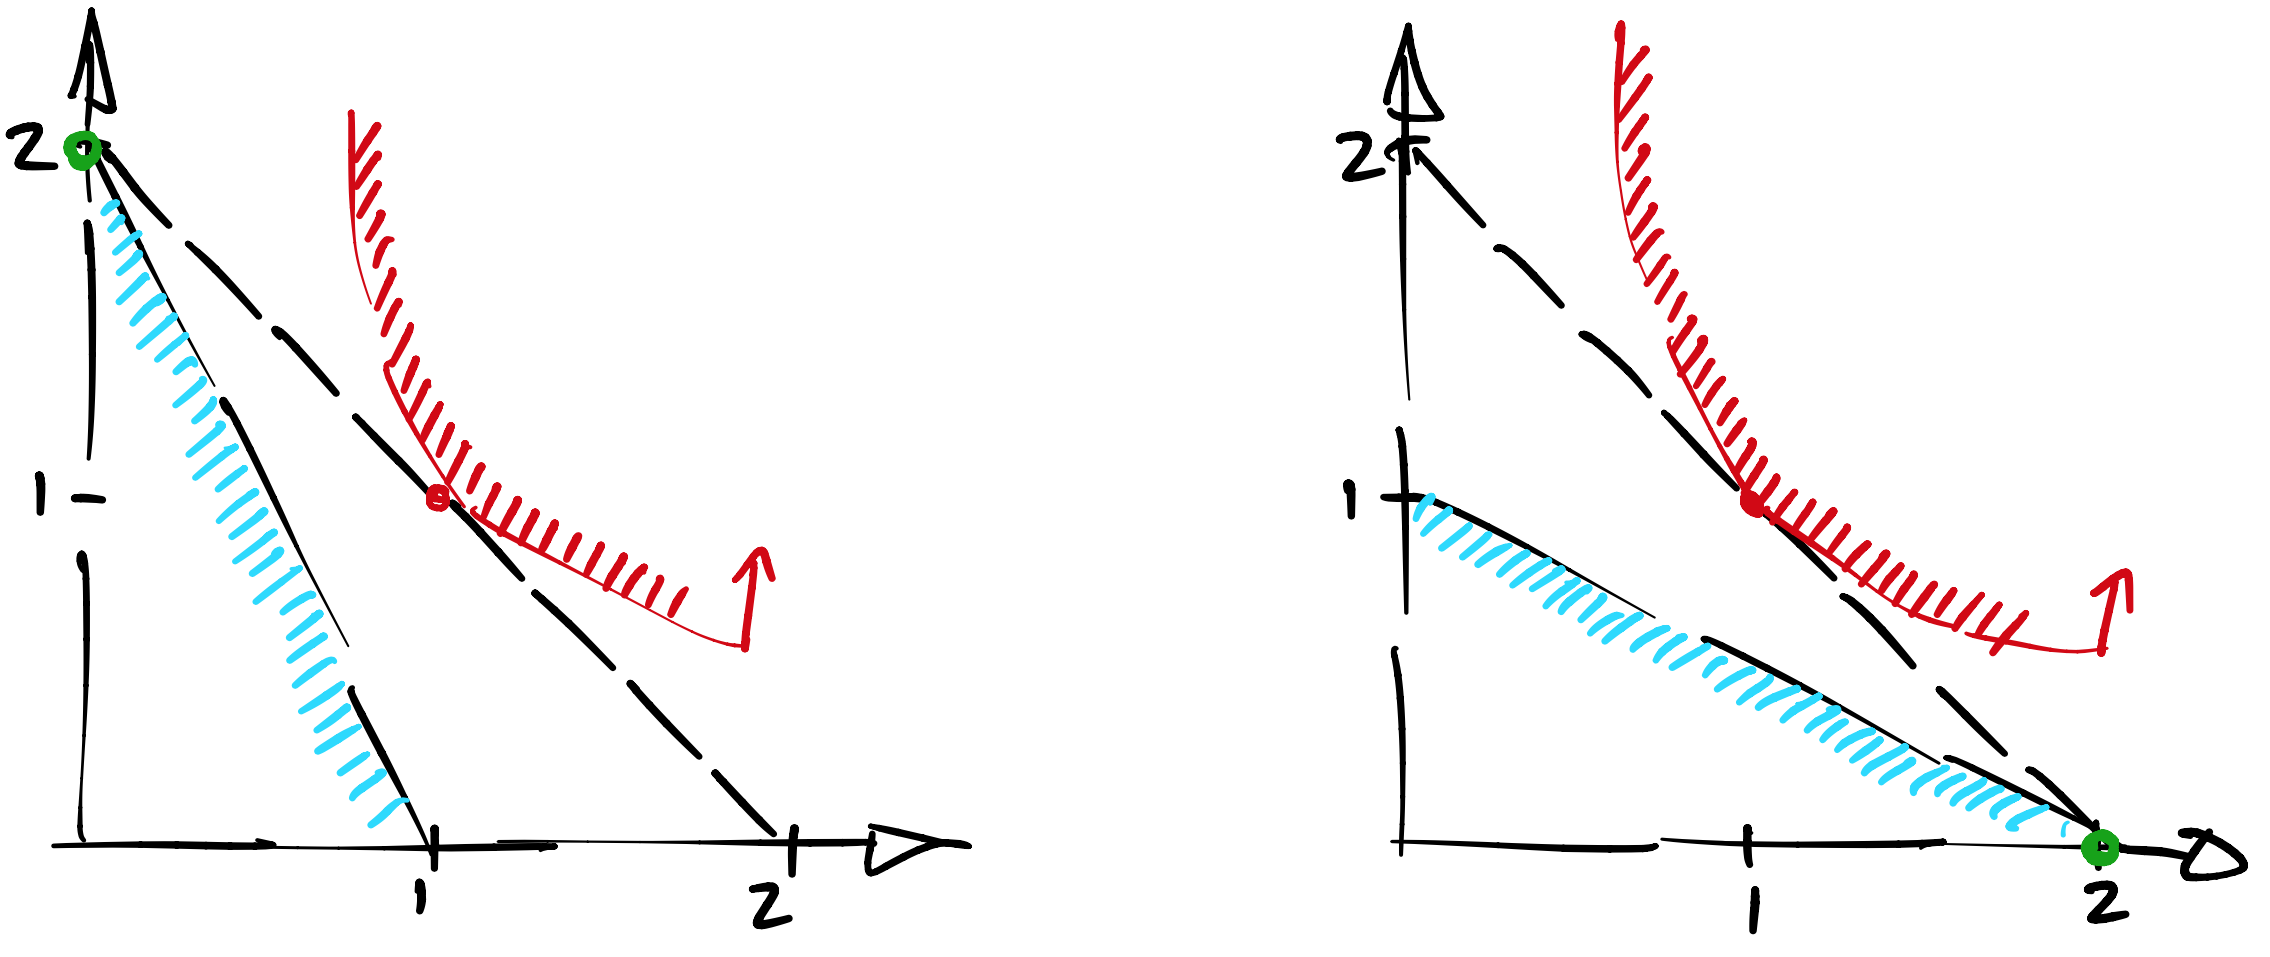
\includegraphics[width=1 \textwidth]{pic2}
\end{figure}

\begin{frame}{Полезность}

Например, у меня на выбор есть

\begin{itemize}
\item 3 куба, 1 круг = 8 утилей
\item 12 конусов = 60 утилей
\item 1 конус, 4 круга = 3 утиля
\end{itemize}

Агенты сравнивают утили и принимают экономические решения, дабы их максимизировать. В данном случае мы выберем 2ой вариант на 60 утилей.

Это самая старая модель, поэтому мы будем называть ее \alert{классической}.

\end{frame}

\begin{frame}{Полезность}

Полезность определена с точностью до монотонного преобразования. Это серьезная проблема, это значит, что модель невозможно толком \alert{откалибровать} или \alert{оценить}.

\end{frame}

\begin{frame}{Полезность}

Действительно, все нижеперечисленные полезности неразличимы с точки зрения наблюдателя. 
\begin{itemize}
\item $x^2 y^3$
\item $2 \log x + 3 \log y$
\item $2 \log x + 3 \log y + 1$
\item $5(2 \log x + 3 \log y) + 1$
\end{itemize}

Если модель нельзя оценить по данным, это однозначно <<плохая>> модель. Экономисты всегда-всегда пытаются от этого избавиться.

\end{frame}

\begin{frame}{Полезность}

Как правило, в классической модели все координаты $x,y$ неотрицательные, потому что непонятно, что значит потребить $-1$ яблок. Это иногда пишется явно, а иногда умалчивается для экономии чернил. 

Всегда подразумеваем что $x,y \geqslant 0$, если не сказано обратное. Но только для потребителя, потому что производитель может потребить -10 яблок, чтобы произвести яблочный сок.

\end{frame}

\begin{frame}{Полезность}

Полезность можно также задать табличкой

\begin{center}
\begin{tabular}{ |c c c| } 
 \hline
 1 яблоко&+ \ 1 груша & = 3 утиля \\ 
 2 яблока&+ \ 1 груша & = 4 утиля \\ 
 1 яблоко&+ \ 2 груши & = 5 утилей \\ 
 \hline
\end{tabular}
\end{center}

Потренируемся в монотонном преобразовании утилей?

\end{frame}


\section{Предпочтения}

\begin{frame}{Предпочтения}

В модели предпочтений от агентов требуется, казалось бы, меньше. Они должны в моменте сравнить два портфеля и назвать лучший. Другими словами, они должны озвучить предпочтения.

Мы будем называть эту модель \alert{неоклассической}.

\end{frame}

\begin{frame}{Предпочтения}

\begin{figure}[hbt]
\centering
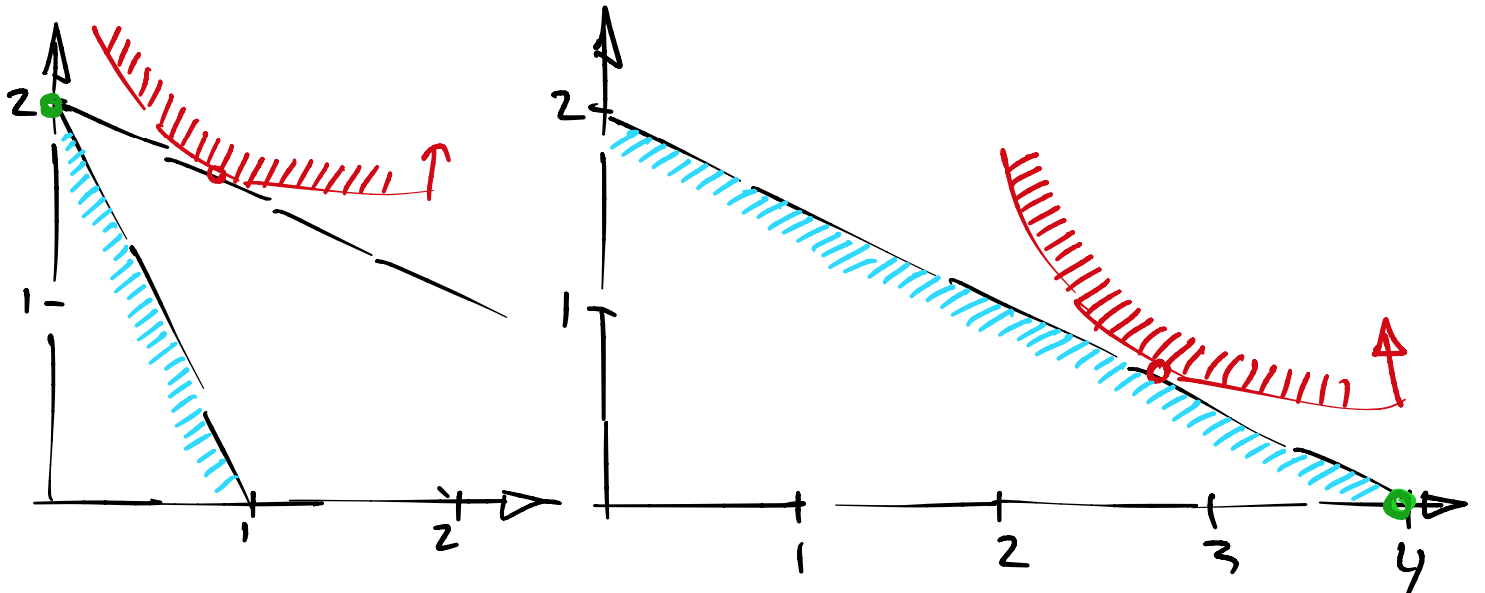
\includegraphics[width=.7 \textwidth]{pic4}
\end{figure}

\end{frame}

\begin{frame}{Предпочтения}

Этот минимализм обманчив. Чтобы оставаться экономическими агентами, они должны помнить все свои выборы, и не менять их на протяжении эксперимента.

Это матрица $n \times n$, где $n$ - это число возможных портфелей. Это очень много надо агенту запомнить.

Зато, здесь отсутствует проблема представления поведения потребителя двумя разными моделями, поэтому экономисты эту модель тоже очень любят.

\end{frame}

\begin{frame}{Предпочтения}

Для простоты пусть есть всего три альтернативы $a,b,c$, тогда я могу зафиксировать выбор таким образом:
$$\begin{array}{c|ccc}
 \succcurlyeq & a & b & c\\
 \hline
 a & 1 & 0 & 1\\
 b & 1 & 1 & 0\\
 c & 1 & 0 & 1
\end{array}$$

Значок $\succcurlyeq$ означает предпочтение. 

Запомним эту таблицу

\end{frame}

\begin{frame}{Предпочтения}

Для данной таблицы $$\succcurlyeq(a,b) = 0, \quad \succcurlyeq(b,a) = 1$$ что означает <<строгое>> предпочтение $b$ над $a$. 

Я буду использовать вот такой значок $b \succ a$ для <<строгого>> и вот такой значок $b \succcurlyeq a$ для <<нестрогого>> предпочтения, что означает
$$\succcurlyeq(a,b) = 0 \text{ или } 1, \quad \succcurlyeq(b,a) = 1$$

... вообще я могу писать просто скобки, без $\succcurlyeq$.

\end{frame}

\begin{frame}{Предпочтения}

Получается довольно элегантный язык предпочтений. 

Ставим в табличку $(x,y) = 1$ если агент проявил нестрогое предпочтение $x$ над $y$, например, добровольно поменял в эксперименте $y$ на $x$.

\begin{itemize}
	\item $(a,b) = 1$ и $(b,a) = 0$ это $a \succ b$
	\item $(a,b) = 0$ и $(b,a) = 1$ это $b \succ a$
	\item $(a,b) = 1$ и $(b,a) = 1$ это $b \sim a$
\end{itemize}

Ставим в табличку $(x,y) = 0$ если (тут нужно проявить фантазию) агент отказался менять $y$ на $x$ плюс <<эпсилон>>.

\end{frame}

\begin{frame}{Предпочтения}

Потренируемся у доски переводить полезности в предпочтения...

Пусть множество альтернатив это числа -2, -1, 0, 1; Заполните матрицу предпочтений для следующих функций полезности, как если бы вы проводили эксперимент над человеком с истинной классической полезностью над целыми числами

\begin{itemize}
\item полезность $x$
\item полезность $x^2$
\item полезность $|x|$
\item полезность $x^3$	
\end{itemize}

\end{frame}

\section{Выбор}

\begin{frame}{Выбор}

В модели выбора от агентов требуется принимать решения, максимально приближенные к реальности. Вам предлагают меню (\alert{menu}) из: $(a,b,c)$, $(a,b)$, $(a,c)$, $(b,c)$, $(a)$, $(b)$, $(c)$.

И вы просто вычеркиваете то, что вам точно не нравится. Все что вы не вычеркнули - это и есть ваш выбор (\alert{choice}). 

Эта модель требует от экономического агента знать не свою функцию полезности, и даже не $n^2$ готовых ответов, как в предпочтениях, а целых $2^n$ готовых ответов.

\end{frame}

\begin{frame}{Выбор}

\begin{figure}[hbt]
\centering
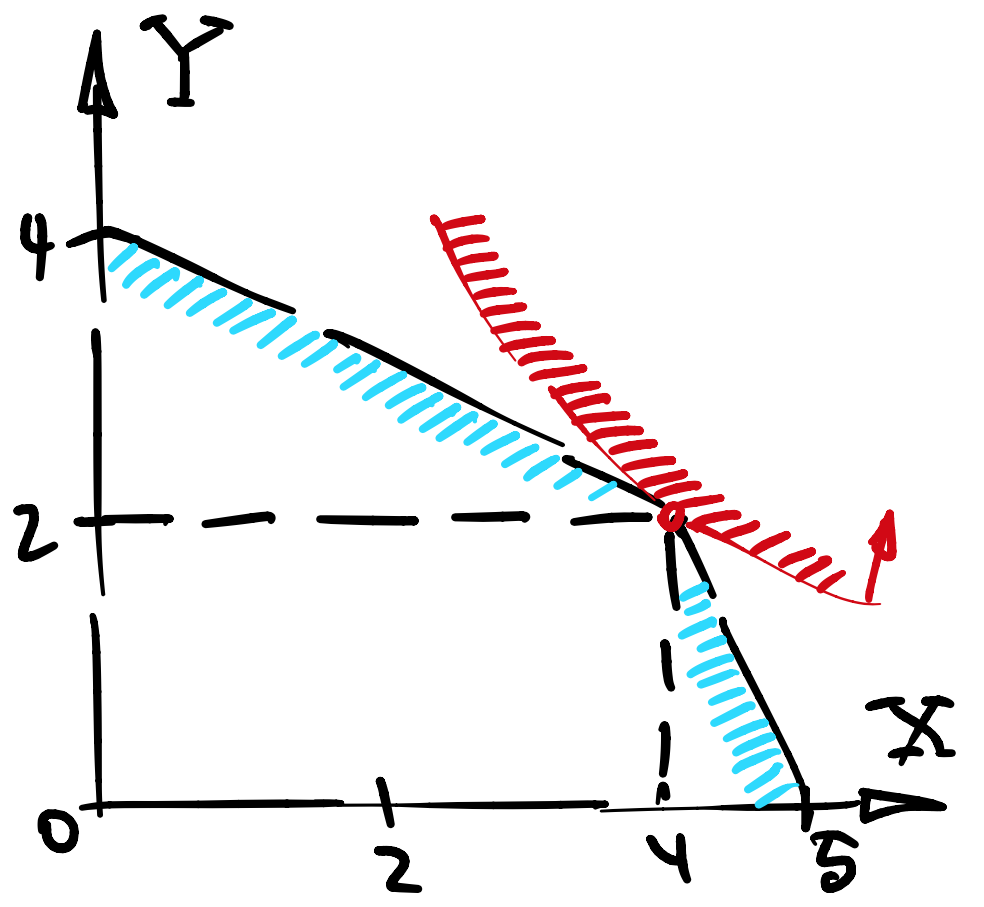
\includegraphics[width=.7 \textwidth]{pic3}
\end{figure}

\end{frame}

\begin{frame}{Выбор}

Потренируемся у доски переводить полезности в выбор...

Пусть меню это наборы (портфели) чисел (-2,1,2), (-1,1), (0,1), (1); Запишите выбор, как если бы вы проводили эксперимент над человеком с истинной классической полезностью над портфелями чисел $\{x_i\}$.

\begin{itemize}
\item полезность $\sum_i x_i$
\item полезность $\sum_i x_i^2$
\item полезность $|x_0|$
\end{itemize}

\end{frame}

\begin{frame}{Выбор}

На самом деле, есть строгие определения того как спускать полезность в предпочтения и предпочтения в выбор (именно такая иерархия) однако я хотел чтобы вы сами догадались, вместо того чтобы запоминать их.

Они очень естественные и интуитивные.
\end{frame}

\section{Какая из моделей лучшая?}

\begin{frame}{Какая из моделей лучшая?}

Можно долго спорить, какая из этих моделей более или менее реалистичная. Правильный ответ - они все нереалистичные. 

\begin{itemize}
  \item агент должен знать ответы на все вопросы
  \item ответ не может меняться во времени
\end{itemize}

Реализм вообще не является добродетелью модели. Вся суть модели в том, чтобы подняться на другой уровень абстракции.
\end{frame}

\section{Потренируемся в моделировании}

\begin{frame}{Потренируемся в моделировании}
	Какую модель вы бы выбрали для описания следующих жизненных задач? и почему

\begin{itemize}
  \item купить продуктов в магазине
  \item выбора университета
  \item голосования в думу
  \item одежду отдать в приют или оставить себе
\end{itemize}	
	
\end{frame}

\begin{frame}{Потренируемся в моделировании}

Предположим, что вы выбрали утилитарную (классическую) модель.

Далее, вам нужно ответить на следующие вопросы

\begin{itemize}
  \item сколько вообще товаром
  \item какие доступны альтернативы
  \item что мы знаем про полезность/предпочтения/выбор
\end{itemize}	
	
\end{frame}

\section{Классическая модель}

\begin{frame}{Классическая модель}

Модель полезности обладает высоким уровнем абстракции

\begin{itemize}
\item начнем с одного агента
\item товары разделены на $n$ категорий
\item портфель/корзина/алътернатива это точка в $\mathbb{R}_{+}^{n}$	
\item категории, а также координаты обозначаются $x, y, z...$
\item соответствующие цены обозначаются $p, q, r...$
\item полезность обозначается $U(x,y,z, \ldots)$
\item множество доступных альтернатив $X \subset \mathbb{R}_{+}^{n}$
\end{itemize}


Плюсик в $\mathbb{R}_{+}^{n}$ означает неотрицательные значения потребления, мы иногда называем это множество \alert{первый/положительный ортант Евклидового пространства}.

\end{frame}

\begin{frame}{Полезность}

Таким образом, мы может сформулировать модель потребителя как абстрактную оптимизационную задачу, скажем, для трех товаров:
$$ U(x,y,z, \ldots) \to \max_{(x,y,z, \ldots) \in X}$$
Формально \alert{классическая  (утилитарная) модель} это пара: множество альтернатив $X \subset \mathbb{R}^n_{+}$ и полезность $U: X \to \mathbb{R}$.

Никаких дополнительных аксиом не требуется.

Множество альтернатив будет, как правило, зависеть от цен $p,q,r...$ и бюджета $W$ (от слова \alert{wage}).
$$ X = \{x,y,z... \in \mathbb{R}_{+}^{n}: p x + q y + r z + \ldots \leqslant W \}$$

\end{frame}

\begin{frame}{Пример 1}

У Пети есть 100 рублей. Он может купить яблоки ($x$) по цене 20 рублей за штуку либо груши ($y$) по цене 50 рублей за штуку. Петя получает полезность 2 за каждое яблоко и 3 за каждую грушу, но не получает никакой полезности за оставшиеся деньги. 

Попробуем записать это формально:

\begin{itemize}
  \item $X = \{(x, y) \in  \mathbb{Z}^2_{+}: 20 x + 50 y \leqslant 100 \}$
  \item $U(x, y) = 2x + 3y$
\end{itemize}

Здесь $\mathbb{Z}^2_{+}$ это \alert{решетка из целых значений}, потому что нельзя покупать нецелые яблоки и груши.

\end{frame}

\begin{frame}{Пример 2}

У Кати есть 24 часа в сутки, из которых она должна как минимум 8 часов поспать ($x$), a дальше она учится и занимается. Однако, на каждый час учебы ($y$) нужен один час отдыха ($z$), и наоборот, иначе время проходит зря.

Попробуем записать это формально:

\begin{itemize}
  \item $X = \{(x, y, z) \in  \mathbb{R}^3_{+}: x + y + z \leqslant 24 \}$
  \item $U(x, y, z) = \mathbb{I}(x \geqslant 8)\cdot \min(y,z)$
\end{itemize}

Здесь $\mathbb{I}(x \geqslant 8)$ это \alert{индикатор-функция}, принимающее значение 1 когда выражение в скобках выполнено, иначе 0.

\end{frame}

\section{Свойства полезности в $\mathbb{R}^n$}

\begin{frame}{Непрерывность}

Мы начнем с двух эквивалентных определений непрерывности.

\begin{definition}
Полезность $U$ \alert{непрерывна} в $X$, если для любого $x \in X$ множества $L_{+}(x)$ и $L_{-}(x)$ замкнуты, где
\begin{gather*} L_{+}(x) = \{y \in X: U(y) \geqslant U(x)\}\\
 L_{-}(x) = \{y \in X: U(y) \leqslant U(x)\}\end{gather*}
\end{definition}

Описанные выше множества $L_{+}(x)$ (или $L_{-}(x)$) - это подмножества допустимых альтернатив, которые не хуже (или не лучше), чем сам $x \in X$. 

Их часто называют \alert{Лебеговыми множествами} относительно точки $x$, $L_{+}(x)$ - верхним а $L_{-}(x)$ - нижним.

\end{frame}

\begin{frame}{Непрерывность}
\centering
рисунок в $\mathbb{R}^{n}$
\begin{figure}[hbt]
\centering
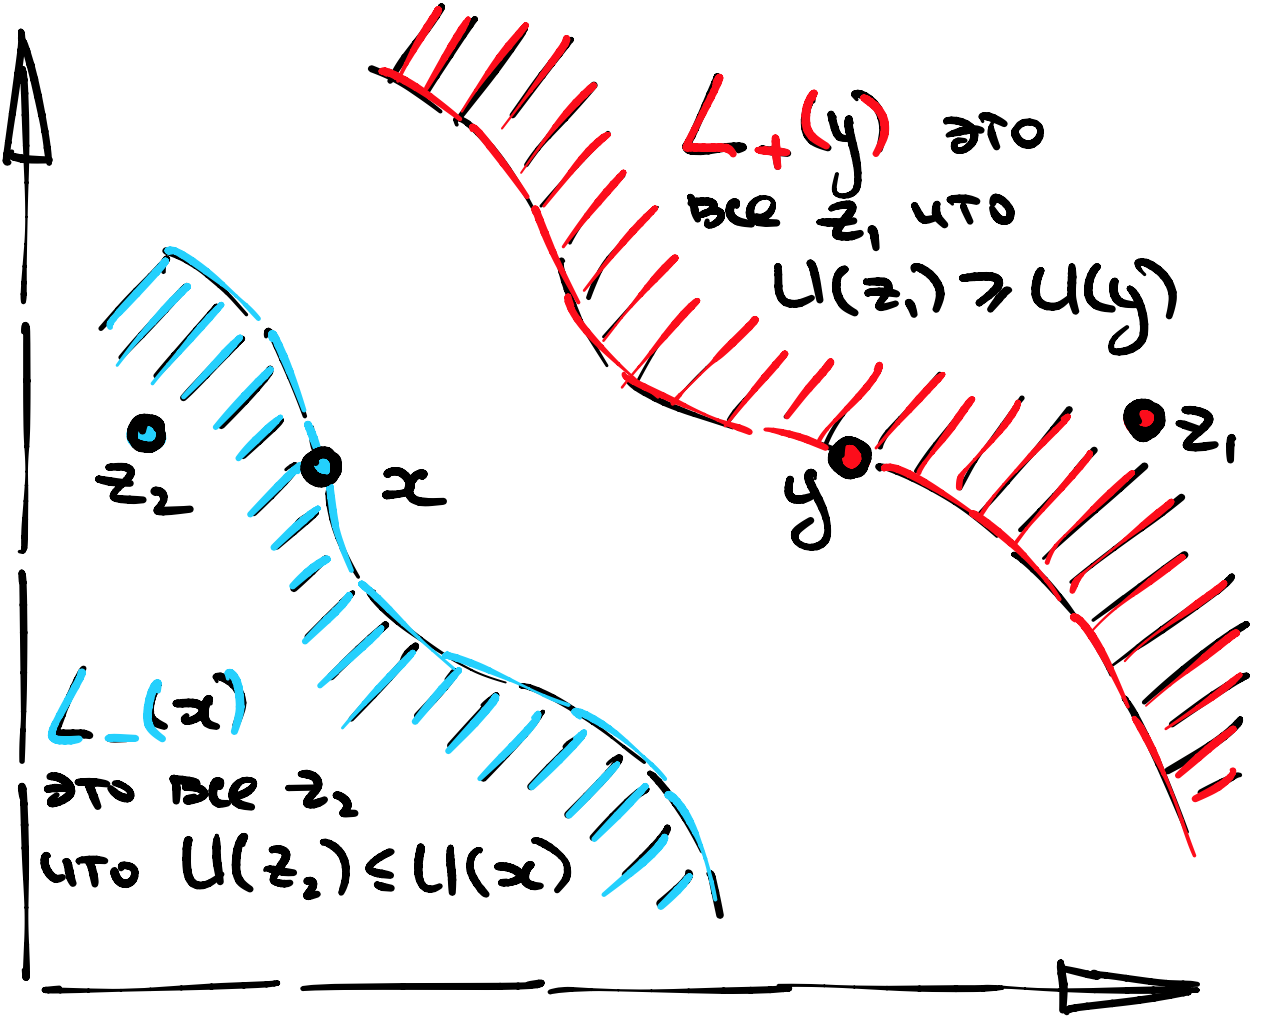
\includegraphics[width=.7 \textwidth]{lebeg_sets.png}
\end{figure}

\end{frame}

\begin{frame}{Непрерывность}

Эквивалентное (но только в Евклидовых пространствах) определение непрерывности можно дать на более знакомом вам с курса мат. анализа языке эпсилон-дельта.

\begin{definition} Полезность $U$ \alert{непрерывна} в $X$, если для любого $\varepsilon > 0$ существует $\delta >0$ такой что для любых $x, y \in X$: $$ ||x - y|| < \delta \quad \Rightarrow \quad ||U(x) - U(y)|| < \varepsilon.$$	
\end{definition}

Но оно практически бесполезно для экономистов.

\end{frame}

\begin{frame}{Вогнутость}

Следующее важное определение - это вогнутость.

\begin{definition}
Полезность $U$ \alert{вогнута}, если для любых $x, y \in X$: 
$$ \forall \alpha \in (0,1): U(\alpha x + (1-\alpha) y)) \geqslant \alpha U(x) + (1-\alpha) U(y)$$
\end{definition}

Многие полезности уже вогнуты сами по себе, например: $ax + by, \min(x,y), \sqrt{xy}, x + \log y$, но некоторые такими не являются, например $\max(x,y)$, $x^2y^2$.

\end{frame}

\begin{frame}{Вогнутость}

\begin{columns}
\begin{column}{0.5\textwidth}
   Пусть пространство товаров $\mathbb{R}^{2}_+$, для простоты. Тогда график функции это такая поверхность. Можно сказать, что \alert{вогнутая функция это когда подграфик выпуклый}, либо, \alert{график вогнутой функции выглядит как колпак}. Еще одно правило - это \alert{график вогнутой функции находится под касательной плоскостью.}\end{column}
\begin{column}{0.5\textwidth}  %%<--- here
    \begin{center}
    рисунок в $\mathbb{R}^{n+1}$
     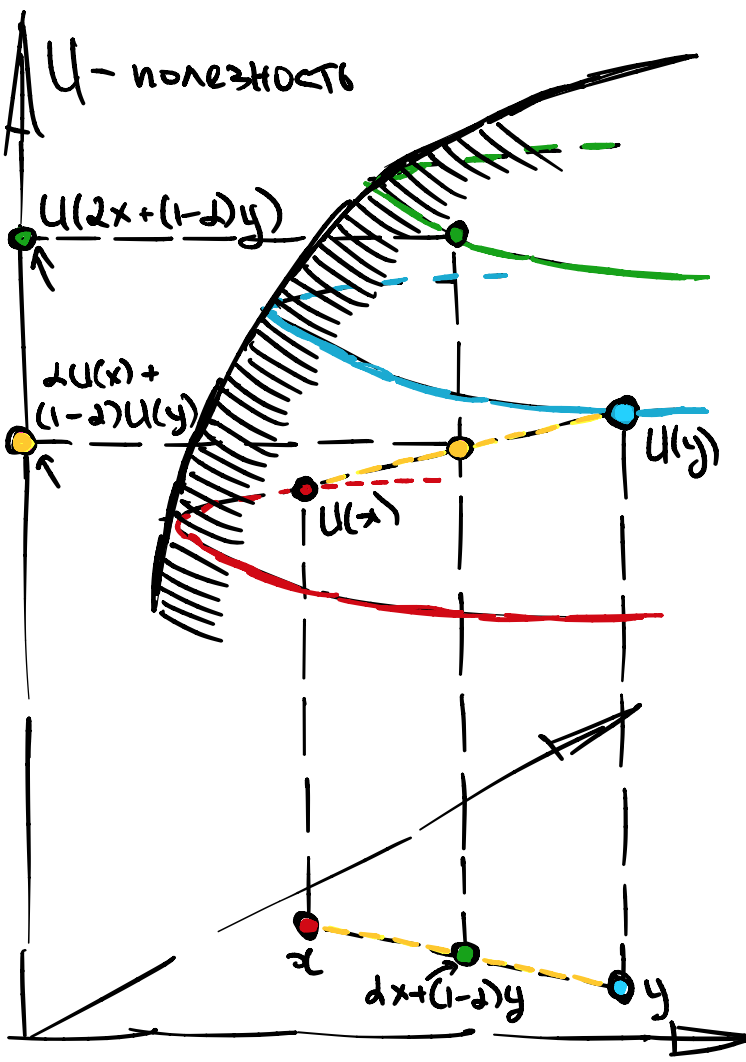
\includegraphics[width=.9\textwidth]{concave.png}
     \end{center}
\end{column}
\end{columns}

\end{frame}

\begin{frame}{Вогнутость}

В этом курсе я буду чаще всего пользоваться 2-мерным (1-мерным) пространством товаров, но когда мне надо будет посмотреть на функцию от этих товаров, будет получаться график в соответственно 3-мерном (2-мерном) пространстве.

\end{frame}


\begin{frame}{Вогнутость}

Постарайтесь не путать ситуацию когда вы смотрите только на область определения функции ($\mathbb{R}^{n}$) где живут верхние и нижние Лебеговы множества, с ситуацией когда вы смотрите на область определения с приклеенной к ней осью утилей ($\mathbb{R}^{n+1}$) где живут график и подграфик функции полезности.

\end{frame}

\end{document}